% ====================================================================
% VİZE RAPOR ŞABLONU – Türk Masalları Derlemesi Web Sayfası
% --------------------------------------------------------------------
% DERLEME: Overleaf'te Menu > Compiler > XeLaTeX (pdfLaTeX de çalışır).
%
% KURALLAR (şablonu kullanmadan önce okuyun):
%  1. Bölüm başlıklarını SİLMEYİN ve sırasını DEĞİŞTİRMEYİN.
%  2. [KÖŞELİ PARANTEZ] içindeki ve gri renkli açıklama metinlerini
%     kendi bilgilerinizle değiştirin; açıklama metinlerini silin.
%  3. MEBİS'e YALNIZCA bu raporun PDF'ini yükleyin.
%     ZIP ve HTML dosyası YÜKLEMEYİN. Tüm kontroller GitHub'dan yapılır.
%  4. Kapaktaki GitHub ve YouTube bağlantıları doğru ve tıklanabilir
%     olmalıdır. Teslimden önce PDF'teki bağlantılara tıklayıp deneyin.
%  5. Haftalık katkı tablosundaki görseller için resim dosyalarını
%     (hafta1.png, hafta2.png, ...) Overleaf projesine yükleyin.
%     Dosya adlarında boşluk ve Türkçe karakter kullanmayın.
%     Resim yoksa tabloda "görsel ekleyin" kutusu görünür.
%  6. Yapay zekâ kullandıysanız Bölüm 5'i doldurun.
% ====================================================================
\documentclass[12pt,a4paper]{article}

\usepackage{iftex}
\ifPDFTeX
  \usepackage[T1]{fontenc}
  \usepackage[utf8]{inputenc}
\else
  \usepackage{fontspec}
\fi
\usepackage[turkish]{babel}
\usepackage[margin=2.4cm]{geometry}
\usepackage{setspace}
\usepackage{graphicx}
\usepackage{booktabs}
\usepackage{longtable}
\usepackage{array}
\usepackage{colortbl}
\usepackage{xcolor}
\usepackage{enumitem}
\usepackage{listings}
\usepackage{amssymb}
\usepackage{caption}
\usepackage{fancyhdr}
\usepackage{hyperref}

\onehalfspacing
\setlength{\parindent}{0pt}
\setlength{\parskip}{6pt}
\setlist{itemsep=2pt, topsep=4pt}
\hypersetup{colorlinks=true, linkcolor=blue!50!black, urlcolor=blue!50!black}

\definecolor{ana}{HTML}{14325C}
\definecolor{acik}{HTML}{EEF2F8}

\lstset{basicstyle=\ttfamily\small, backgroundcolor=\color{acik},
  frame=single, rulecolor=\color{ana}, breaklines=true,
  columns=fullflexible, keepspaces=true, showstringspaces=false}

\pagestyle{fancy}
\fancyhf{}
\fancyhead[L]{EVVEL ZAMAN}
\fancyhead[R]{Vize Raporu}
\fancyfoot[C]{\thepage}

% ---------- Yardımcı komutlar ----------
% Gri açıklama metni (silinecek yönergeler için)
\newcommand{\aciklama}[1]{{\color{gray}\itshape (#1)}}

% Haftalık tablo görseli: dosya yoksa "görsel ekleyin" kutusu çıkar
\newcommand{\haftagorsel}[1]{%
  \IfFileExists{#1}{%
    \includegraphics[width=\linewidth,height=4.2cm,keepaspectratio]{#1}%
  }{%
    \fbox{\parbox[c][2.6cm][c]{\dimexpr\linewidth-2\fboxsep-2\fboxrule\relax}{%
      \centering\small\color{gray} Ekran görüntüsü / görsel ekleyin\\ \texttt{#1}}}%
  }%
}
% Haftalık katılım kutuları (işaretlemek için $\square$ yerine $\boxtimes$ yazın)
\newcommand{\katilimkutulari}{\par\vspace{3pt}\small $\square$ Ders içinde katılım sergiledim\par $\square$ Telafi yaptım}

% Ek görsel: dosya yoksa hiçbir şey göstermez
\newcommand{\haftaek}[1]{%
  \IfFileExists{#1}{\\[4pt]\includegraphics[width=\linewidth,height=4.2cm,keepaspectratio]{#1}}{}%
}

% ---------- Kapak bilgileri ----------
\newcommand{\universite}{İSTANBUL MEDİPOL ÜNİVERSİTESİ / GÖRSEL İLETİŞİM TASARIMI BÖLÜMÜ}
\newcommand{\dersadi}{PROGRAMLAMAYA GİRİŞ}
\newcommand{\hocaadi}{MERAL ŞENTÜRK}
\newcommand{\ogrenciadi}{MERYEM KARATAŞ}
\newcommand{\ogrencino}{86240010}
\newcommand{\projeadi}{EVVEL ZAMAN}
% Bağlantıları tam adres olarak yazın (https:// ile başlayarak)
\newcommand{\githublink}{\url{https://github.com/meryemkaratas997-ai/Evvel-Zaman-Web-Site}}
\newcommand{\youtubelink}{\url{https://youtu.be/gHq4Zxiqwsg}}

\begin{document}

% ====================================================================
% KAPAK
% ====================================================================
\begin{titlepage}
\centering
\vspace*{1cm}
{\large \universite \par}
\vspace{1.8cm}
{\Huge\bfseries\color{ana} \projeadi \par}
\vspace{0.4cm}
{\Large Türk Masalları Derlemesi Web Sayfası \par}
{\large Vize Raporu \par}
\vspace{1.8cm}
{\large \textbf{Ders:} \dersadi \par}
{\large \textbf{Öğretim Üyesi:} \hocaadi \par}
\vspace{1.2cm}
{\large \textbf{Hazırlayan:} \ogrenciadi \par}
{\large \textbf{Öğrenci No:} \ogrencino \par}
\vspace{1.8cm}
\fbox{\parbox{0.88\linewidth}{\centering\vspace{6pt}
{\large\bfseries Proje Bağlantıları}\\[8pt]
\textbf{GitHub deposu:}\\ \githublink \\[8pt]
\textbf{YouTube sunum videosu:}\\ \youtubelink
\vspace{6pt}}}
\vfill
{\large \today \par}
\end{titlepage}

\tableofcontents
\newpage

% ====================================================================
\section{Giriş}
% ====================================================================
\aciklama Bu projede amacım, geleneksel Türk masallarını modern ve etkileşimli bir web arayüzünde toplayarak kullanıcılara keyifli bir dijital okuma deneyimi sunmaktır. Masalların dijital ortamda kaybolmasını önlemek, okuyucunun aradığı masala kolayca ulaşmasını sağlamak ve okuma sürecini kişisel notlar, alıntılar ile incelemelerle daha dinamik hale getirmek için bu uygulamayı geliştirdim. Ödev gereksinimleri doğrultusunda projemde toplam 8 adet özgün halk masalına yer verdim. Dışarıdan herhangi bir ek kütüphane veya harici dosya bağımlılığı olmadan, tüm yapıyı tek bir .html dosyası içinde kurguladım. Sayfa düzeni ve responsive tasarımı <style> etiketleri arasına yazdığım içsel (internal) CSS ile sağlarken; filtreleme, tema değişimi ve yerel veri kaydı gibi tüm dinamik işlevleri de <script> blokları içindeki saf (vanilla) JavaScript kodlarıyla eksiksiz şekilde karşıladım. Bu raporda ise uygulamanın temel mimarisini, veri yapılarını, kullanıcı etkileşimlerini ve teknik çözüm süreçlerimi adım adım ele aldım.

\subsection{Proje Özeti}
Evvel Zaman, Türk masallarını modern ve kullanıcı odaklı bir arayüzde bir araya getiren tek sayfalık bir web uygulamasıdır. Kullanıcılar sol tarafta yer alan katalog üzerinden 8 farklı masal arasından seçim yapabilmekte, arama kutusu ve kategori etiketlerini kullanarak masalları anlık olarak filtreleyebilmektedir. Seçilen masal sağdaki okuma panelinde görüntülenirken; yazı boyutu ayarlama, gece/gündüz modu seçeneği ve okuma durumu belirleme (okudum, okuyorum, daha sonra oku) gibi özellikler sunulmaktadır. Ayrıca okuyucular metin içinden doğrudan cümle seçerek alıntı kaydedebilmekte ve masallara 1–5 arası yıldız verip inceleme yazabilmektedir. Sayfanın profil sekmesinde ise kullanıcının okuma istatistikleri, aldığı alıntılar ve masallara yaptığı değerlendirmeler düzenli bir şekilde listelenmektedir.

\subsection{Gereksinimlerin Karşılanması}
\begin{center}
\rowcolors{2}{acik}{white}
\begin{tabular}{@{}p{8.2cm}c@{}}
\toprule
\rowcolor{ana}\textcolor{white}{\textbf{Gereksinim}} & \textcolor{white}{\textbf{Durum}} \\
\midrule
Masal sayısı 8--12 arasında ([SAYI] masal)         & $\boxtimes$ \\
Tek HTML dosyası                                    & $\boxtimes$ \\
Stil kodları içsel (\texttt{<style>} içinde)        & $\boxtimes$ \\
Betik kodları içsel (\texttt{<script>} içinde)      & $\boxtimes$ \\
İnternetsiz açılıp çalışıyor                        & $\boxtimes$ \\
JavaScript sayfada anlamlı bir işlev görüyor        & $\boxtimes$ \\
Masal metinleri kendi cümlelerimle yazıldı          & $\square$ \\
Sayfa telefonda da düzgün görünüyor                 & $\boxtimes$ \\
\bottomrule
\end{tabular}
\end{center}

% ====================================================================
\section{Masalların Seçimi}
% ====================================================================

\begin{longtable}{@{} c >{\raggedright\arraybackslash}p{3.2cm} >{\raggedright\arraybackslash}p{2.6cm} >{\raggedright\arraybackslash}p{7.8cm} @{}}
\toprule
\textbf{No} & \textbf{Masal} & \textbf{Tür} & \textbf{Seçilme nedeni} \\
\midrule
\endhead
1 & Tuz Kadar Sevmek & Gerçekçi masal & Sevginin değerini sabır ve emek üzerinden anlatan, halk anlatılarındaki klasik tuz motifiyle güçlü bir hayat dersi veren yapısı için seçtim. \\
2 & Nardaniye Hanım & Olağanüstü Masal & Ay ile konuşma, zehirlenme ve dirilme gibi zengin fantastik motifleriyle Türk halk edebiyatının en köklü anlatı kalıplarından birini temsil ettiği için seçtim. \\
3 & Üç Turunçlar & Olağanüstü Masal & Büyülü meyveler, şekil değiştirme (güvercin, ağaç, beşik) ve dev kalesi gibi katmanlı masal motiflerini çok canlı aktardığı için seçtim. \\
4 & Telli Turna & Olağanüstü Masal & Kuş-insan dönüşümü üzerinden Karadeniz doğasını ve sevgi, masumiyet gibi felsefi temaları modern bir dille birleştirdiği için seçtim. \\
5 & Hüsnü Yusuf & Olağanüstü Masal & Peri padişahının oğlu, güvercin donuna girme ve tılsımlı nesneler gibi halk kültürünün olağanüstü unsurlarını barındırdığı için seçtim. \\
6 & Dürümcekli Kadın Masalı & Hayvan Masalı & Hayvan kahramanlar arasındaki komik diyaloglar, tekerlemeler ve mizahi kurgusuyla derlemeye farklı bir tür zenginliği katması için seçtim. \\
7 & Mitişik Kız & Olağanüstü Masal & Dev anası figürüne karşı fiziksel güç yerine kıvrak zekâ ve akılla kurulan tuzakları anlatan tipik bir kurnazlık masalı olduğu için seçtim. \\
8 & Uyusun, Uyansın da Güllere Boyansın & Gerçekçi Masal & Güç sahibi bir padişaha karşı genç bir kadının hazırcevaplığı, aklı ve rengârenk güller motifiyle meydan okumasını işlediği için seçtim. \\
\bottomrule
\end{longtable}

% ====================================================================
\section{Tasarım Kararları}
% ====================================================================
\aciklama 
Bu projede herhangi bir hazır şablon veya kütüphane (Bootstrap vb.) kullanmadan, doğrudan masal okuma deneyimini geliştirmeye odaklanan özgün bir arayüz tasarladım. Ekranı solda masal kataloğu, sağda ise okuma alanı olacak şekilde iki bölmeli  kurgulayarak kullanıcının sayfadan kopmadan masallar arasında hızlıca geçiş yapmasını sağladım; mobil cihazlarda ise bu yapıyı dikey düzene uyarlayarak akışı korudum. Tasarımın genelinde eski kitap sayfalarını andıran krem tonları ile geleneksel kiremit kırmızısını kullanarak masal atmosferini dijital ortama yansıttım. Okuma ergonomisini desteklemek adına metinlerde gözü yormayan tırnaklı bir yazı tipi (Georgia), buton ve kontrollerde ise sade bir yazı tipi tercih ettim; ayrıca ilk harf vurgusu ile klasik kitap hissiyatını güçlendirdim. Okuyucunun göz konforu için satır uzunluğunu ideal okuma sınırı olan yaklaşık 72 karakterde tuttum, gece modu seçeneği ve yazı boyutunu dinamik olarak değiştiren kontroller (A+ / A-) ekledim. Son olarak alıntı kaydetme ve inceleme yazma gibi etkileşimli alanları doğrudan masalın altına entegre ederken, kullanıcı profili panelini ayrı bir alanda gizleyerek sayfanın sade kalmasını ve dikkatin tamamen okuma deneyiminde yoğunlaşmasını sağladım.

\subsection{Konuya Uygunluk}
Projenin renk, yazı tipi ve genel düzen tercihlerini Türk masallarının köklü anlatı geleneğini dijital ortama yansıtacak biçimde belirledim. Sayfa zemininde modern soğuk beyazlar yerine eski el yazması kitapları ve sararmış kâğıt dokusunu çağrıştıran sıcak parşömen tonlarını, vurgularda ise geleneksel minyatür ve çini sanatını andıran kiremit kırmızısını kullanarak tematik bir atmosfer oluşturdum. Masalların yüzyıllar öncesine dayanan yapısını hissettirmek ve uzun soluklu okumalarda göz yorgunluğunu önlemek amacıyla gövde metinlerinde tırnaklı yazı tipi tercih ettim; ilk paragraflarda kullandığım büyük harf vurgusuyla da klasik masal kitaplarındaki başlangıç süslemelerine gönderme yaptım. Arayüz butonları ve filtrelerde ise sade, modern bir font kullanarak okunabilirliği dengede tuttum. Sayfayı dikkati dağıtan hazır resimlerle doldurmak yerine okuma deneyimini ve okuyucunun hayal gücünü ön planda tuttum; masal temasına uygun görsel kişiselleştirmeyi ise yalnızca profil alanında kullanıcıya sunduğum peri kızı, şehzade, padişah veya turna gibi masalsı avatar seçenekleriyle sade bir şekilde sağladım.
\subsection{Renk Paleti ve Yazı Tipi}
\begin{center}
\rowcolors{2}{acik}{white}
\begin{tabular}{@{} l l >{\raggedright\arraybackslash}p{8cm} @{}}
\toprule
\rowcolor{ana}\textcolor{white}{\textbf{Ad}} & \textcolor{white}{\textbf{Kod}} & \textcolor{white}{\textbf{Nerede / neden kullandınız?}} \\
\midrule
Parşömen / Sıcak Krem & \texttt{[\#f6f3ea]} & Sayfa arka planında kullandım. Saf ve soğuk beyaz yerine eski kitap sayfalarını andıran sıcak bir zemin yaratarak masal temasını desteklemek ve göz yorgunluğunu azaltmak için seçtim. \\
Kiremit Kırmızısı & \texttt{[\#943328]} & Başlıklarda, butonlarda, aktif sekmelerde ve kenarlıklarda vurgu rengi olarak kullandım. Geleneksel Türk el sanatlarını ve çini tonlarını çağrıştırdığı, arayüzde önemli yerleri net şekilde öne çıkardığı için tercih ettim. \\
Koyu Kömür / Metin Rengi & \texttt{[\#2b2725]} & Başlık ve gövde metinlerinde kullandım. Sert siyah yerine hafif yumuşatılmış koyu bir ton seçerek krem arka plan üzerinde yüksek okunabilirlik ve dengeli bir kontrast sağladım. \\
Açık Bej / Sınır Çizgisi & \texttt{[\#e5dfd3]} & Kart kenarlıklarında, ayırıcı çizgilerde ve buton çerçevelerinde kullandım. Sayfadaki bölümleri gözü yormadan ve sert hatlar oluşturmadan birbirinden ayırmak için tercih ettim. \\
Georgia, Palatino, serif & -- & Masal metinlerinin gövdesinde kullandım. Tırnaklı yapısıyla klasik basılı kitap hissiyatı vermek ve uzun metinlerde gözün satır takibini kolaylaştırmak için seçtim. \\
Sistem Sans-Serif & -- & Menülerde, butonlarda, arama kutusunda ve profil panelinde kullandım. Kullanıcı arayüzü kontrollerinin modern, sade ve ekran boyutuna bakılmaksızın kolayca okunabilmesi için tercih ettim. \\
\bottomrule
\end{tabular}
\end{center}

\subsection{Okunabilirlik, Gezinme ve Duyarlı Tasarım}
\begin{itemize}
  \item \textbf{Okunabilirlik:} Masal gövdesinde gözü dinlendiren 18 piksellik temel yazı boyutu tercih ettim ve kullanıcının isteğine göre boyutu değiştirebileceği kontroller (A+ / A-) ekledim. Uzun satırların okumayı zorlaştırmasını engellemek için metin bloğunu en fazla 72 karakter (max-width: 72ch) ve 1.85 satır yüksekliğiyle sınırlandırdım. Sıcak krem zemin üzerine koyu tonlu yazı rengi kullanarak gözü yormayan yüksek bir kontrast elde ettim, karanlık modda ise parlamayı önleyen koyu arka plan ve yumuşak açık metin renkleriyle gece okumasını rahatlattım.
  \item \textbf{Gezinme:} Kullanıcı istediği masala sol tarafta yer alan masal kataloğundaki kartlara tek tıkla basarak sayfayı yenilemeden anında ulaşabilmektedir. Ayrıca başlıkta bulunan dinamik arama çubuğu sayesinde masal adı, özeti veya motifine göre anlık arama yapabilmekte; kategori butonlarıyla da masalları türlerine göre kolayca filtreleyebilmektedir.
  \item \textbf{Duyarlı tasarım:} Geniş ekranlı bilgisayarlarda ekran solda 340 piksellik masal listesi, sağda ise okuma alanı olacak şekilde iki sütunlu (CSS Grid) bir yapıda açılmaktadır. Ekran genişliği 900 pikselin altına (tablet ve telefonlara) indiğinde ise CSS medya sorguları devreye girerek bu iki bölmeyi tek sütunlu alt alta bir akışa dönüştürmekte, seçilen masal otomatik olarak ekranın üst kısmına kayarak mobil cihazlarda rahat bir okuma sağlamaktadır.
  \item \textbf{Tutarlılık:} Tüm sayfada renkler ve gölgeler CSS değişkenleri (:root) üzerinden merkezi bir sistemle yönetilerek her bileşende aynı tonların kullanılması sağlandı. Başlık hiyerarşisi belirli ölçülerle (h1, h2, h3) korunmuş; butonlar, kartlar ve form alanlarında standart 6–8 piksellik köşe yuvarlama (border-radius) ve 12–24 piksellik boşluklar kullanılarak arayüzde görsel bir bütünlük oluşturulmuştur.
\end{itemize}

\subsection{Ekran Görüntüleri}

\begin{center}
\resizebox{11cm}{!}{
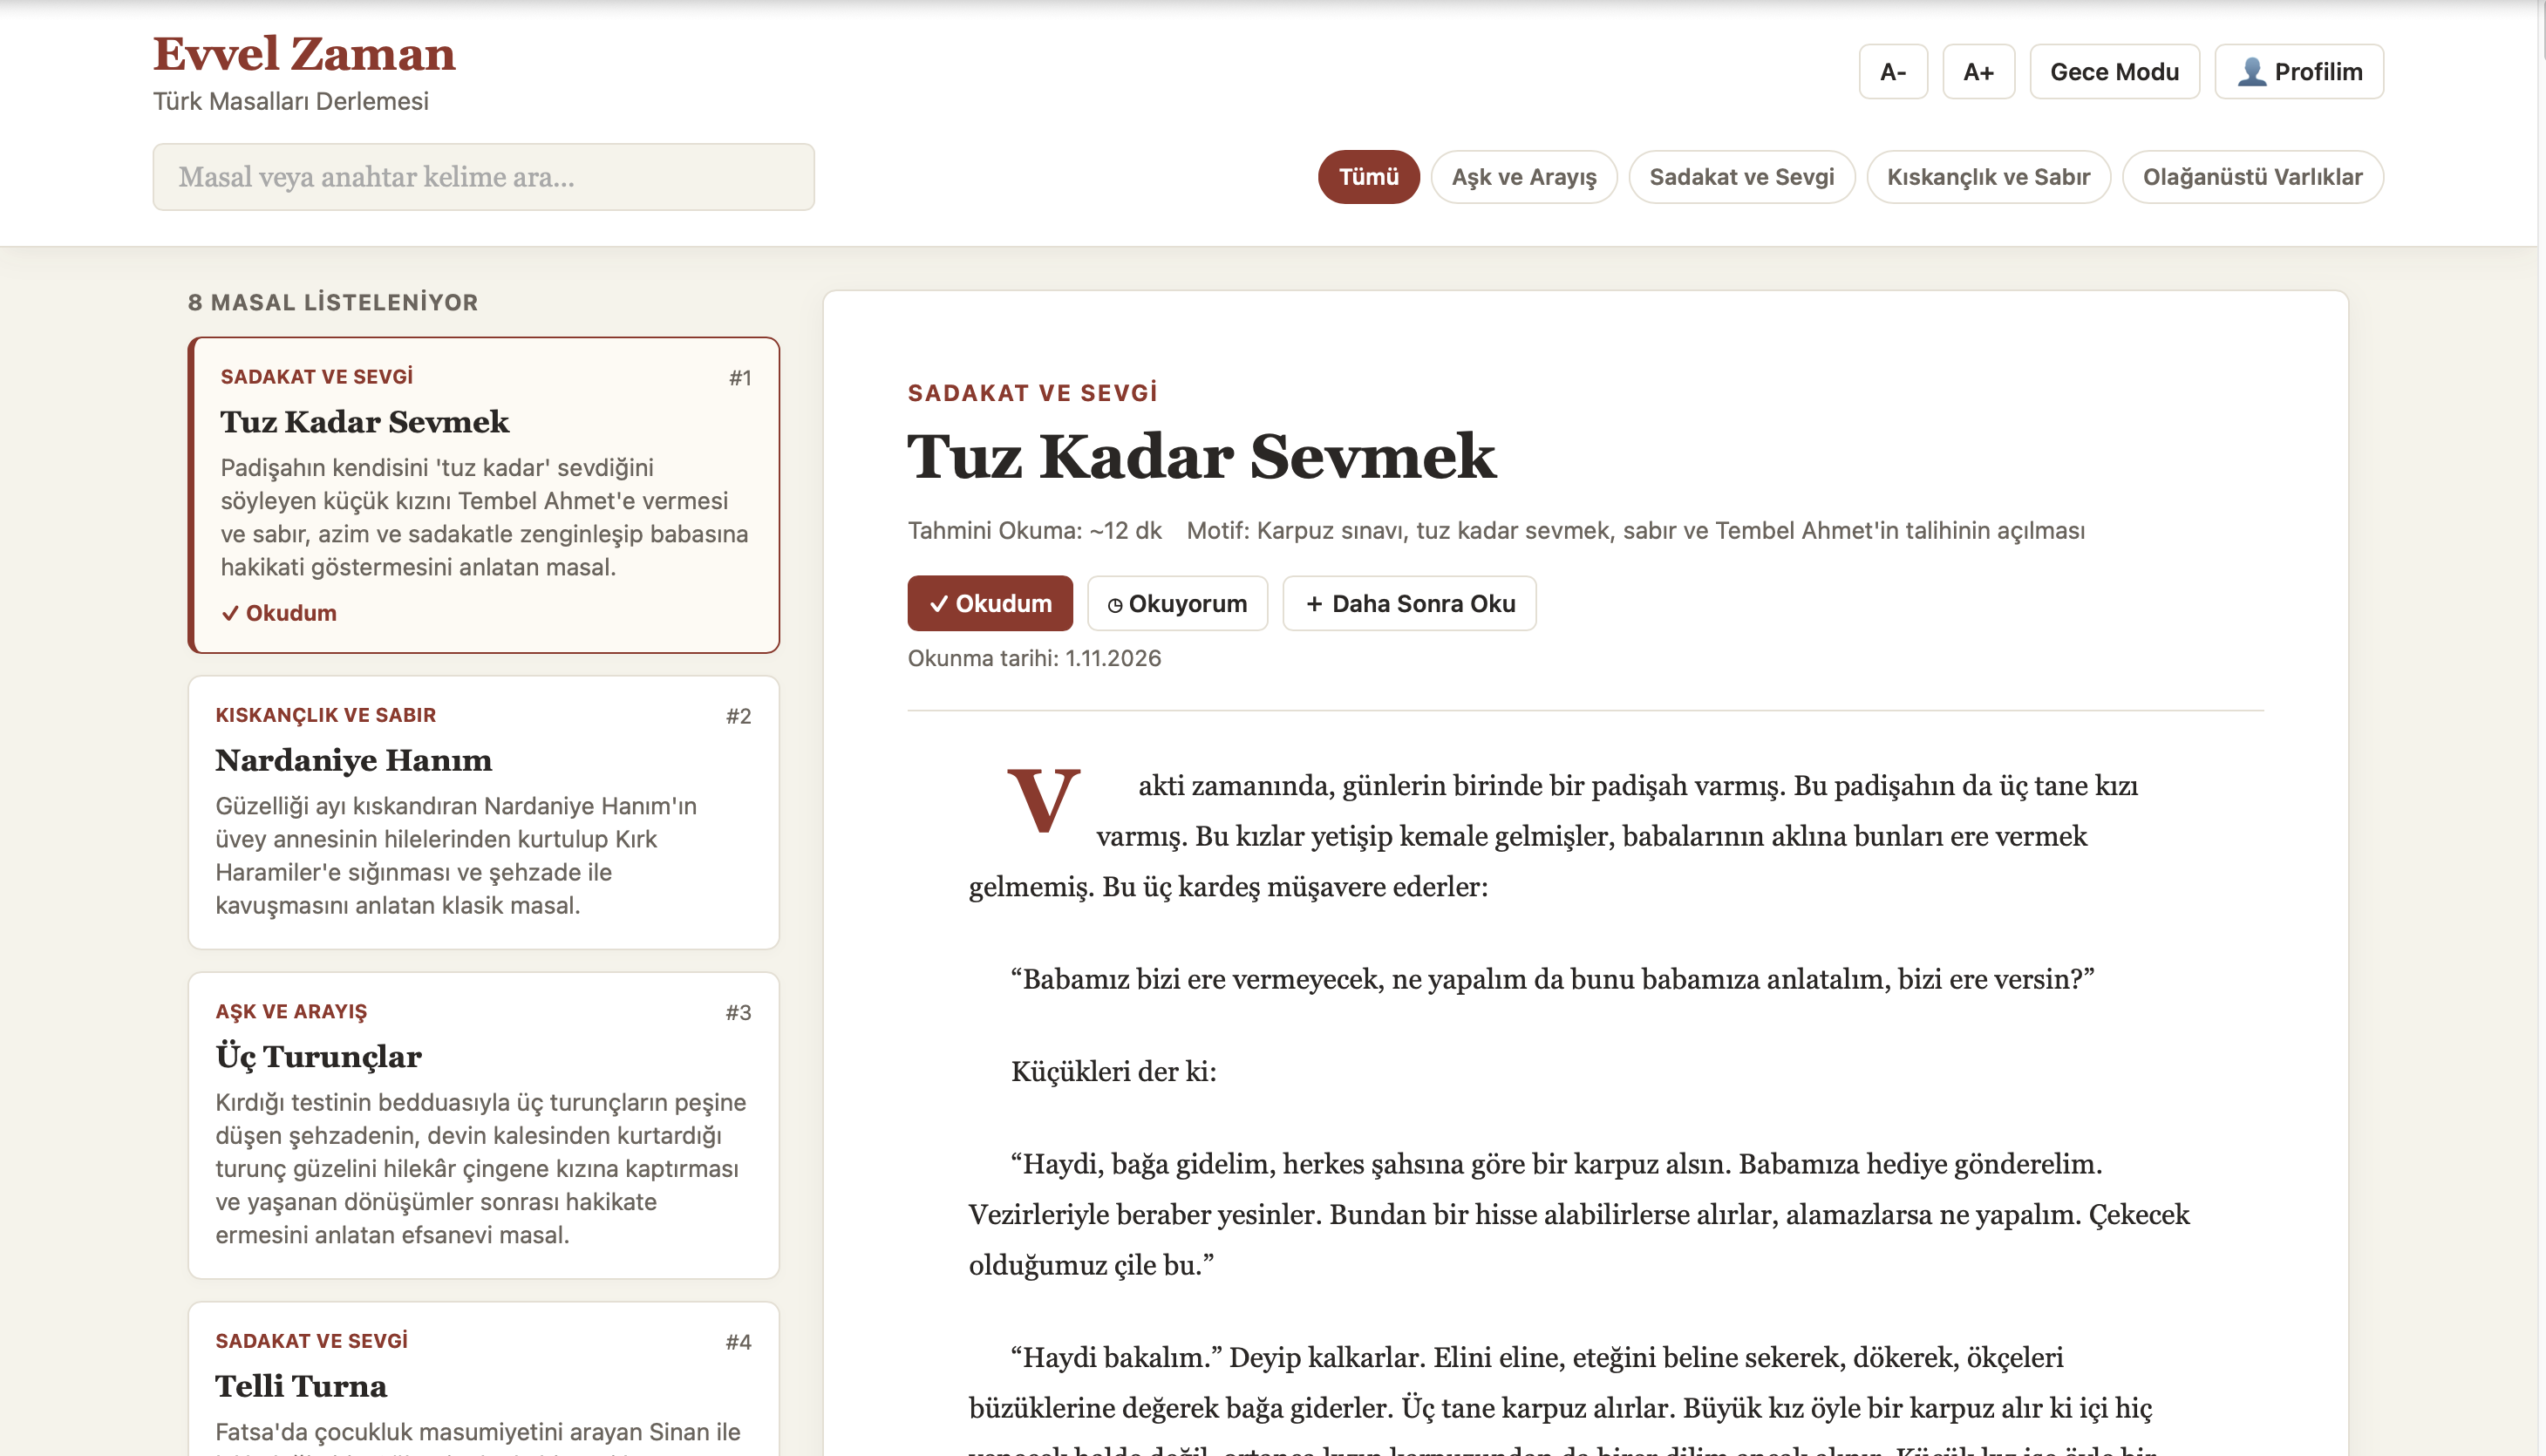
\includegraphics{ekran-masaustu.png}
}

\vspace{4pt}
\small\textbf{Şekil 1:} Sayfanın bilgisayar görünümü
\end{center}
\begin{center}
\resizebox{5.5cm}{!}{
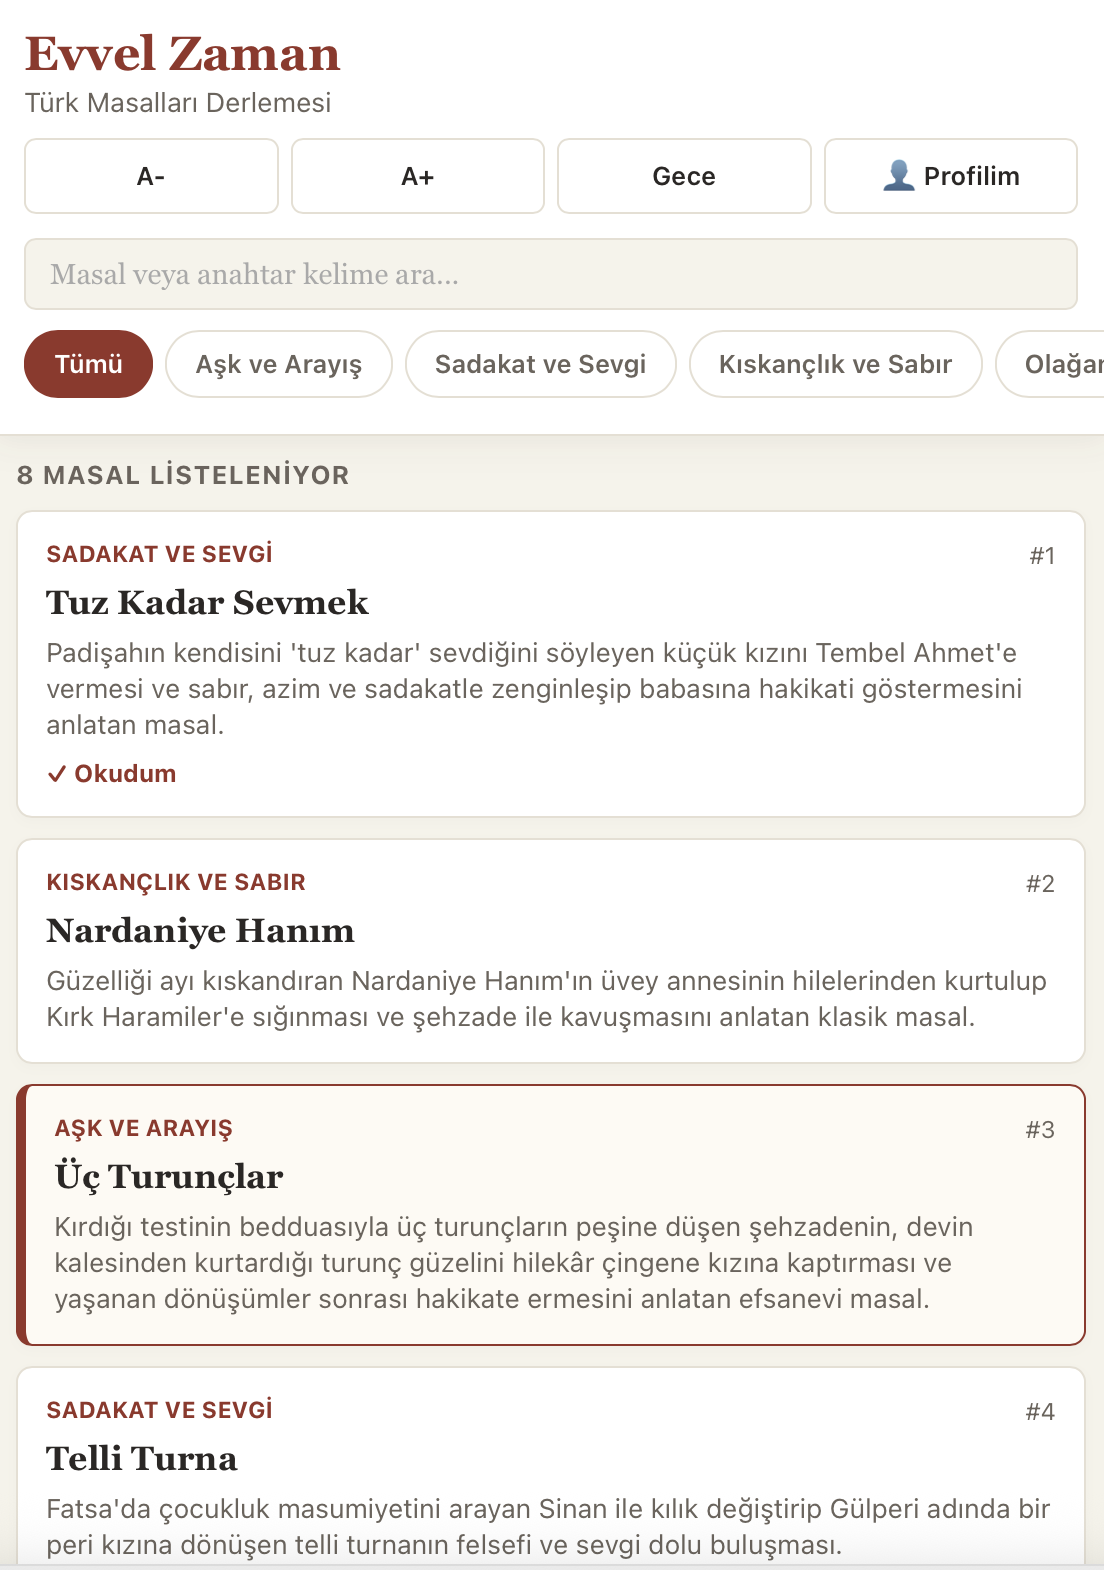
\includegraphics{ekran-mobil.png}
}

\vspace{4pt}
\small\textbf{Şekil 2:} Sayfanın telefon görünümü
\end{center}

% ====================================================================
\section{Gerçekleştirme}
% ====================================================================
\aciklama 
Uygulamam tek bir HTML dosyası üstünden çalışıyor ve kullanıcı işlem yaptıkça sayfa hiç yenilenmeden ekran JavaScript ile güncelleniyor. Sayfa ilk açıldığında tarayıcının hafızasına (localStorage) bakıp daha önceden kaydedilmiş okuma durumlarını, notları veya tema ayarını hemen yüklüyor.
Kod tarafında uyguladığım mantığı ve önemli yerleri şu şekilde özetleyebilirim:
1. Verileri Saklama Şekli: Bütün masalları TALES adında bir dizi içinde nesne olarak tuttum. Her masalın id’si, adı, kategorisi ve paragrafları bu yapıda duruyor:
1. Verileri Saklama Şekli: Bütün masalları TALES adında bir dizi içinde nesne olarak tuttum. Her masalın id'si, adı, kategorisi ve paragrafları bu yapıda duruyor:
\begin{verbatim}
const TALES = [
  { id: 1, title: "Tuz Kadar Sevmek", category: "Sadakat ve Sevgi",
    paragraphs: ["Vakti zamanında..."] }
];
\end{verbatim}

3. Masali Ekrana Basma: Soldaki masallardan birine tiklandiginda selectTale fonksiyonu calisiyor ve secilen masalin paragraflarini arayuzdeki okuma alanina basiyor:
\begin{verbatim}
function selectTale(id) {
  const tale = getTale(id);
  viewText.innerHTML = tale.paragraphs.map(p => p).join('');
}
\end{verbatim}

4. Metinden Alinti Alma: Okurken fareyle bir cumle secildiginde tarayicinin secim ozelligiyle o cumleyi yakalayip uzerine tiklandiginda not ekleten kucuk bir alinti butonu cikartiyorum:
\begin{verbatim}
const selection = window.getSelection();
const text = selection ? selection.toString().trim() : '';
\end{verbatim}

5. Verileri Kaydetme: Okudugum masallari, yazdigim yorumlari ve alintilari tek bir yerde toplayip localStorage icine atiyorum. Boylece sayfa kapansa bile yazdiklarim silinmiyor:
\begin{verbatim}
function saveData() {
  localStorage.setItem('STORAGE_KEY', JSON.stringify(data));
}
\end{verbatim}

\subsection{HTML Yapısı}
Sayfamın iskeletini anlamsal HTML5 etiketlerini kullanarak ekranın işlevlerine göre mantıksal bölümlere ayırdım. En üstte yer alan <header> bölümünde uygulamanın ana başlığı (<h1>), kısa açıklama metni ile profil ve gece modu butonları bulunmaktadır. Masalların aranması ve filtrelenmesi için <input type="search"> ile kategori butonlarını barındıran bir filtreleme alanına yer verdim. Sayfanın gövdesini oluşturan <main> etiketini iki ana bölüme ayırdım; sol taraftaki <aside> etiketinde masal kartlarının dinamik olarak listelendiği katalog yer alırken, sağ taraftaki <section> etiketinde seçilen masalın başlığı (<h2>), detay bilgileri, yazı boyutu kontrolleri ve paragrafların basıldığı okuma alanı bulunmaktadır. Yine bu okuma bölümünün hemen devamında okuma durumu butonları, kaydedilen alıntılar ve yıldızlı değerlendirme formu (<form>) yer almaktadır. Metinden cümle seçildiğinde açılan alıntı penceresi ile masalcı profil paneli için gizlenebilir arayüz yapıları (<div>, <textarea>) kullanırken, sayfanın en altında ise kaynakça ve künye bilgilerini taşıyan <footer> etiketine yer verdim.

\subsection{İçsel CSS}
Sayfamın tüm stillerini harici bir kütüphane kullanmadan \texttt{<style>} etiketi içerisinde içsel CSS (internal CSS) olarak yazdım. Aldığım önemli stil kararları ve kodumdan örnekler şu şekildedir:

\begin{itemize}
\item \textbf{CSS Değişkenleri (:root):} Renk paletini ve tema ayarlarını tek bir merkezden yönetmek için değişkenler tanımladım. Bu sayede karanlık modda sadece bu değişkenlerin değerlerini ezerek sitenin tüm temasını kolayca değiştirebildim:
\end{itemize}

\begin{lstlisting}[caption={CSS Değişkenleri ve Tema Ayarları}]
:root {
  --bg-page: #f6f3ea;
  --text-main: #2b2725;
  --accent-primary: #943328;
  --border-color: #e5dfd3;
}

body.dark-mode {
  --bg-page: #1f1b18;
  --text-main: #eae3d9;
}
\end{lstlisting}

\begin{itemize}
\item \textbf{Sayfa Düzeni (CSS Grid ve Flexbox):} Ana yerleşimde sol katalog paneli ile sağ okuma alanını yan yana konumlandırmak için iki sütunlu CSS Grid kullandım. Buton grupları, arama alanı ve başlık gibi bileşenlerin hizalanmasında ise Flexbox tercih ettim:
\end{itemize}

\begin{lstlisting}[caption={Grid ve Flexbox Yerlesimi}]
/* Ana iki bolmeli yerlesim */
.app-layout {
  display: grid;
  grid-template-columns: 340px 1fr;
  gap: 24px;
}

/* Butonlar ve kontroller icin esnek dizilim */
.header-actions, .category-chips {
  display: flex;
  align-items: center;
  gap: 10px;
}
\end{lstlisting}

\begin{itemize}
\item \textbf{Duyarlı Tasarım Kuralları (Responsive Design):} Ekran genişliği 900 pikselin altına indiğinde yan yana duran Grid yapısını tek sütuna çevirerek telefon ve tabletlerde bölümlerin alt alta düzgün akmasını sağladım:
\end{itemize}

\begin{lstlisting}[caption={Mobil ve Tablet Uyumlu Media Query}]
@media (max-width: 900px) {
  .app-layout {
    grid-template-columns: 1fr;
    gap: 16px;
  }
}
\end{lstlisting}

\begin{itemize}
\item \textbf{Tipografi ve Okuma Ergonomisi:} Masal metinlerinin gözü yormaması ve basılı kitap hissi vermesi için maksimum satır genişliği belirledim ve ilk harf vurgusu (drop cap) ekledim:
\end{itemize}

\begin{lstlisting}[caption={Tipografi ve İlk Harf Vurgusu}]
.tale-content {
  font-family: Georgia, Palatino, serif;
  line-height: 1.85;
  max-width: 72ch;
}

.tale-content p:first-of-type::first-letter {
  font-size: 2.8rem;
  float: left;
  line-height: 1;
  padding-right: 8px;
  color: var(--accent-primary);
}
\end{lstlisting}

\subsection{İçsel JavaScript}
Sayfamın dinamik çalışmasını sağlayan tüm JavaScript kodlarını harici bir dosya bağlamadan, HTML dosyasının en altına \texttt{<script>} etiketleri arasına yazdım. Kod yapımı üç temel başlıkta özetleyebilirim:

\begin{enumerate}
\item \textbf{Masal Verisinin Tutulma Şekli (JSON/Dizi Yapısı):} Masallara ait tüm bilgileri tek tek HTML'e yazmak yerine \texttt{TALES} adında bir JavaScript dizisi (array) içinde tuttum. Her masal; \texttt{id}, \texttt{title}, \texttt{category}, \texttt{readingTime}, \texttt{motif} ve paragraflarını barındıran birer nesne olarak tanımlandı:
\end{enumerate}

\begin{lstlisting}[caption={TALES Veri Yapısı}]
const TALES = [
  {
    id: 1,
    title: "Tuz Kadar Sevmek",
    category: "Sadakat ve Sevgi",
    readingTime: "12 dk",
    paragraphs: ["Vakti zamaninda bir padisah varmis...", "Kucuk kizi der ki..."]
  }
  // ... diger 7 masal
];
\end{lstlisting}

\begin{enumerate}
\setcounter{enumi}{1}
\item \textbf{Temel Fonksiyonlar ve Görevleri:}
\begin{itemize}
  \item \texttt{filterTales()}: Arama çubuğuna yazılan metni ve seçilen kategoriyi kontrol eder; \texttt{filter()} ve \texttt{includes()} metotlarıyla uyuşan masalları bulup ekrandaki listeyi anlık yeniler.
  \item \texttt{renderList(list)}: Filtrelenmiş veya tüm masalları sol taraftaki katalog paneline kartlar halinde dinamik olarak basar.
  \item \texttt{selectTale(id)}: Listeden bir masala tıklandığında çalışır; seçilen masalın başlığını, süresini ve paragraflarını sağdaki okuma alanına aktarır.
  \item \texttt{saveData()} ve \texttt{loadData()}: Kullanıcının okuma durumlarını, aldığı alıntıları ve yorumları \texttt{localStorage} üzerine \texttt{JSON.stringify} ile kaydeder veya açılışta \texttt{JSON.parse} ile geri yükler.
\end{itemize}

\item \textbf{Olayların (Event Listeners) Bağlanması:} Sayfadaki etkileşimleri yakalamak için JavaScript'in \texttt{addEventListener} metodunu kullandım:
\begin{itemize}
  \item \textbf{Arama ve Filtre:} Arama kutusuna \texttt{input} olayı bağlayarak her harf yazıldığında dinamik filtreleme sağladım:
\end{itemize}
\end{enumerate}

\begin{lstlisting}[caption={Olay Dinleyicileri (Event Listeners)}]
searchInput.addEventListener("input", (e) => {
  searchQuery = e.target.value;
  filterTales();
});
\end{lstlisting}

\begin{itemize}
  \item \textbf{Masal Seçimi ve Butonlar:} Dinamik oluşan masal kartlarına \texttt{click} olayı vererek \texttt{selectTale(id)} fonksiyonunu tetikledim.
  \item \textbf{Alıntı Alma (Selection API):} Okuma alanına \texttt{mouseup} olayı bağladım; kullanıcı fareyle metinden bir cümle seçtiğinde \texttt{window.getSelection()} ile cümleyi yakalayıp üzerinde alıntı butonunu açtım.
  \item \textbf{Form Gönderimi:} Masalın altındaki inceleme formuna \texttt{submit} olayı bağlayarak sayfanın yenilenmesini \texttt{e.preventDefault()} ile engelledim ve verileri kaydettim.
\end{itemize}

\subsection{Sayfanın Özellikleri}


% ====================================================================
\section{Yapay Zekâ Kullanımı}

\begin{longtable}{@{}p{1.8cm}p{2.2cm}p{5.5cm}p{4.5cm}@{}}
\toprule
\textbf{Arac} & \textbf{Ne icin kullandiniz?} & \textbf{Istem ozeti} & \textbf{Sayfada nerede?} \\
\midrule
\endhead

Gemini & Kod & Okudum, Okuyorum ve Daha Sonra Oku butonlari ile okuma durumlarinin yonetimi ve localStorage kaydi & Okuma paneli altindaki durum kontrol butonlari (.status-group) ve JS durum fonksiyonlari \\
\midrule
Gemini & Kod & Metinden cumle secilince acilan Alintila butonu (Selection API) ve kullanicilarin masallara yildiz ve yorum yazdigi inceleme formu yapisi & Okuma alanindaki metin secimi (mouseup), alinti ekleme modali ve masal alti inceleme formu (reviewForm) \\
\midrule
Gemini & Kod ve Arayuz & Kullanicinin okuma yuzdesini, okudugu masallari, alintilari ve incelemelerini topluca gosteren Profilim modal ekraninin tasarimi ve istatistik hesaplama mantigi & Ust menudeki Profilim butonu, profil acilir penceresi (profileModal) ve JavaScript profil fonksiyonlari \\
\midrule
Gemini & Kod ve Metin & 8 Turk halk masalinin JSON veri yapisina (TALES) aktarilmasi ve arama-filtreleme algoritmasi & JavaScript script blogundaki masal veri havuzu ve arama cubugu (filterTales) \\
\bottomrule
\end{longtable}

\subsection{Anladığım ve Kendim Yaptığım Kısımlar}
Yapay zekâyı projeyi doğrudan yaptırmak için değil, kafamdaki fikirleri koda dökebilmek için bir rehber ve geliştirme aracı olarak kullandım. Günlük hayatımda 1000Kitap uygulamasını aktif olarak kullanıyorum ve oradaki okuma deneyimini çok sevdiğim için sitemde de benzer bir yapının olmasını istedim. Masalları ``Okudum'', ``Okuyorum'', ``Daha Sonra Oku'' şeklinde ayırma fikrini, metinden alıntı seçip kaydetme özelliğini, masalların altına inceleme yazıp yıldız verme sistemini ve profil sayfasında okuma oranını yüzde olarak görme mantığını yapay zekâya ben sundum ve adım adım kodlattım. Kodlar geldikten sonra tarayıcımın konsolunda (Console) testler yaparak butonların çalışıp çalışmadığını ve verilerin tarayıcıya (\texttt{localStorage}) doğru kaydedilip kaydedilmediğini tek tek denedim. Görsel tasarım tarafında ise yapay zekânın verdiği sade ve ruhsuz şablonu tamamen değiştirdim; masal atmosferine yakışması için sıcak parşömen arka planını (\texttt{\#f6f3ea}), kiremit kırmızısı vurguları (\texttt{\#943328}), tırnaklı (serif) kitap fontlarını ve eski kitap hissi veren o ilk harf büyüklüğü (drop cap) detayını CSS kodlarına kendim ekledim.
\section{Haftalık Katkılar}
% ====================================================================


\begin{longtable}{@{}>{\raggedright\arraybackslash}p{1.7cm}%
                    >{\raggedright\arraybackslash}p{6.4cm}%
                    >{\centering\arraybackslash}p{6cm}@{}}
\toprule
\rowcolor{ana}\textcolor{white}{\textbf{Hafta}} & \textcolor{white}{\textbf{Yapılan çalışma}} & \textcolor{white}{\textbf{Görsel}} \\
\midrule
\endfirsthead
\toprule
\rowcolor{ana}\textcolor{white}{\textbf{Hafta}} & \textcolor{white}{\textbf{Yapılan çalışma}} & \textcolor{white}{\textbf{Görsel}} \\
\midrule
\endhead
\bottomrule
\endfoot

\textbf{1. hafta}\newline 16 Eylül & 
Ders kapsamında verilen ilk HTML şablonu üzerinde çalıştım. Sayfanın temel tipografi kurallarını, başlık stillerini ve arka plan renklerini CSS ile düzenleyerek bağlantıların (\texttt{<a>}) ve metinlerin renk paletini değiştirdim.\newline 
\textbf{Commit:} İlk HTML/CSS düzenlemesi ve renk paleti uyarlaması\newline
$\boxtimes$ Ders içinde katılım sergiledim.\newline
$\square$ Telafi yaptım & 
\haftagorsel{hafta1.png}\haftaek{hafta1b.png} \\
\midrule
\textbf{2. hafta}\newline 23 Eylül & 
Şermin Yaşar'ın biyografisini ve eserlerini tanıtan tek sayfalık bir web sayfası hazırladım. Sayfaya semantik \texttt{<header>}, \texttt{<nav>}, \texttt{<main>} ve \texttt{<section>} etiketlerini entegre ettim; \texttt{<figure>} ve \texttt{<img>} etiketleriyle görsel ekleyip CSS ile görsel boyutunu ve hizalamasını düzenledim.\newline 
\textbf{Commit:} Biyografi sayfası yapısı ve görsel entegrasyonu\newline
$\boxtimes$ Ders içinde katılım sergiledim.\newline
$\square$ Telafi yaptım & 
\haftagorsel{hafta2.png}\haftaek{hafta2b.png} \\
\midrule
\textbf{3. hafta}\newline 30 Eylül & 
JavaScript ile temel kullanıcı etkileşimlerini ve olay dinleyicilerini (\texttt{addEventListener}) uyguladım. Butonlara tıklama (\texttt{click}, \texttt{onclick}) ve fare hareketi (\texttt{mousemove}) olayları bağlayarak uyarı pencereleri (\texttt{alert}) açtırdım; bağlantı etiketleri ve \texttt{window.open} fonksiyonu ile sayfaların aynı veya yeni sekmede açılmasını sağladım.\newline 
\textbf{Commit:} JavaScript temel fare olayları ve sekme yönlendirmeleri\newline
$\boxtimes$ Ders içinde katılım sergiledim.\newline
$\square$ Telafi yaptım & 
\haftagorsel{hafta3.png}\haftaek{hafta3b.png} \\
\midrule
\textbf{4. hafta}\newline 7 Ekim & 
Kullanıcıdan girdi alma ve DOM elemanlarını dinamik olarak güncelleme pratikleri yaptım. \texttt{<input>} alanından metin okuyup boşluk kontrolü yaparak ekrana karşılama mesajı yazdırdım; ayrıca artır ve azalt butonlarıyla değişken değerini değiştirip sonucu anlık olarak \texttt{<p>} etiketine basan bir sayaç mekanizması kodladım.\newline 
\textbf{Commit:} Form girdisi okuma, veri doğrulama ve sayaç uygulaması\newline
$\boxtimes$ Ders içinde katılım sergiledim.\newline
$\square$ Telafi yaptım & 
\haftagorsel{hafta4.png}\haftaek{hafta4b.png} \\
\midrule
\textbf{5. hafta}\newline 14 Ekim & 
Derste paylaşılan renk eşleme ve sayfa yönlendirme kodları üzerinde çalıştım. Kodun CSS kısmında kartların boyutlarını, kenar boşluklarını ve kutuların varsayılan arka plan renklerini değiştirerek arayüzü kişiselleştirdim; buton tıklamasıyla \texttt{window.location.href} kullanarak sayfalar arası geçiş mantığını denedim.\newline 
\textbf{Commit:} Renk eşleme şablonunda kutu boyutları, renk düzenlemeleri ve sayfa yönlendirmesi\newline
$\square$ Ders içinde katılım sergiledim.\newline
$\boxtimes$ Telafi yaptım & 
\haftagorsel{hafta5.png}\haftaek{hafta5b.png} \\
\midrule
\textbf{6. hafta}\newline 21 Ekim & 
CodePen şablonları üzerinden JavaScript ile koşullu durum (\texttt{if-else}) yapısını ve harici CSS bağlama mantığını inceledim. Butona tıklandığında kutunun rengini dinamik olarak değiştiren kod üzerinde denemeler yaparak kutunun ve sayfanın arka plan renkleri ile metin renklerini kişiselleştirdim.\newline 
\textbf{Commit:} JavaScript koşullu renk değişimi ve harici CSS stil uyarlamaları\newline
$\square$ Ders içinde katılım sergiledim.\newline
$\boxtimes$ Telafi yaptım & 
\haftagorsel{hafta6.png}\haftaek{hafta6b.png} \\

\end{longtable}

% ====================================================================
\section{Test ve Değerlendirme}
% ====================================================================
Sayfayı macOS üzerindeki masaüstü Safari tarayıcısında ve iPhone üzerindeki mobil Safari tarayıcısında test ettim. Bilgisayar ortamında Safari üzerinde masalların listelenmesi, arama kutusu, alıntı alma, gece modu, profil ekranı ve \texttt{localStorage} kayıtları eksiksiz ve sorunsuz çalıştı. Ancak sayfa mobil Safari üzerinde açıldığında butonlar ve temel arayüz elemanları ekranda görünmesine rağmen butonlara tıklanamadı ve hiçbir işlem tetiklenmedi; ayrıca seçilen masalın gövde metni ekrana hiç yüklenmedi. Bu durumun temel nedeni; kodlarımızın fare olaylarına (\texttt{click}, \texttt{mouseup}) göre kurgulanmış olması, dokunmatik ekran olaylarının (\texttt{touchstart}/\texttt{touchend}) tanımlanmamış olması ve mobil tarayıcıda JavaScript kodunun ilk yükleme anında masal metnini DOM'a aktarırken hata alıp sonraki betiklerin çalışmasını durdurmasıdır.

\begin{center}
\rowcolors{2}{acik}{white}
\begin{tabular}{@{}p{6.5cm}p{2.5cm}p{5.5cm}@{}}
\toprule
\rowcolor{ana}\textcolor{white}{\textbf{Özellik}} & \textcolor{white}{\textbf{Bilgisayar}} & \textcolor{white}{\textbf{Telefon}} \\
\midrule
Sayfa Arayüzü ve Butonların Görünürlüğü & Çalışıyor & Çalışıyor (Arayüz ve butonlar ekranda görünüyor) \\
Masal Metninin Yüklenmesi ve Gösterimi & Çalışıyor & Sorun var (Masal metni alana basılmıyor, okuma alanı boş kalıyor) \\
Buton Etkileşimleri (Tıklama / Dokunma) & Çalışıyor & Sorun var (Butonlar ekranda görünmesine rağmen tıklanamıyor ve tepki vermiyor) \\
Dinamik Arama ve Kategori Filtreleme & Çalışıyor & Sorun var (Arama alanı ve butonlar dokunmatik olarak tetiklenmiyor) \\
Okuma Durumları (Okudum / Okuyorum / Sonra Oku) & Çalışıyor & Sorun var (Butonlara basılamadığı için durum seçimi yapılamıyor) \\
Alıntı Alma & Çalışıyor & Sorun var (Metin yüklenmediği ve seçim tetiklenmediği için çalışmıyor) \\
İnceleme Formu ve Profil Penceresi & Çalışıyor & Sorun var (Açma ve gönderme butonları dokunmaya yanıt vermiyor) \\
Verilerin Saklanması & Çalışıyor & Sorun var (Butonlar tetiklenmediği için veri akışı ve kayıt gerçekleşmiyor) \\
\bottomrule
\end{tabular}
\end{center}

\textbf{Denenen tarayıcılar:} Safari (macOS ve iOS)
% ====================================================================
\section{Sunum Videosu}
% ====================================================================
\begin{center}
\begin{tabular}{@{}ll@{}}
\textbf{Video süresi:} & [16:52] \\
\textbf{Görünürlük:} & [ Herkese açık] \\
\textbf{Bağlantı:} & \ https://youtu.be/gHq4Zxiqwsg \\
\end{tabular}
\end{center}

\subsection{Video Kontrol Listesi}
\begin{itemize}
  \item[$\boxtimes$] Süre 12--18 dakika aralığında.
  \item[$\boxtimes$] Sunum boyunca kameram açık, yüzüm görünüyor.
  \item[$\square$] Görünürlük \textbf{Listelenmemiş} (ya da Herkese açık); \textbf{Özel} değil.
  \item[$\square$] Bağlantıyı gizli pencerede açtım, video oynuyor.
  \item[$\boxtimes$] YouTube videoyu işlemeyi bitirdi.
  \item[$\boxtimes$] Videoyu baştan sona izledim; ses ve kamera tüm sunumda var.
  \item[$\boxtimes$] Kapaktaki bağlantı ile bu bölümdeki bağlantı aynı.
\end{itemize}

% ==============================================================================
\section{Sonuç ve Kendi Değerlendirmem}
% ==============================================================================

Bu proje sayesinde temel HTML, içsel CSS ve JavaScript mekanizmalarının birbirleriyle nasıl haberleştiğini ve dinamik bir web arayüzünün nasıl inşa edildiğini uygulamalı olarak öğrendim. Özellikle verileri bir JSON dizisinde tutup DOM üzerinden ekrana dinamik basma mantığını ve \texttt{localStorage} kullanarak kullanıcı etkileşimlerini tarayıcı hafızasında saklamayı deneyimledim. En çok zorlandığım nokta, metin üzerinden cümle seçildiğinde çalışan Selection API mekanizmasını kurmak ve Türkçe karakter uyumlu arama algoritmasını kurgulamak oldu. Bu sorunları tarayıcının geliştirici konsolunda hataları adım adım takip ederek ve arama fonksiyonunu \texttt{toLocaleLowerCase("tr-TR")} ile güncelleyerek çözdüm. Sayfanın masaüstü Safari ortamında sorunsuz çalışmasına rağmen, mobil Safari'de butonların tıklanmaması ve masal metninin ekrana gelmemesi sürecin en büyük eksikliğiydi. İleride bu projeyi geliştirecek olursam, öncelikle dokunmatik ekranlara özel dokunma olaylarını (\texttt{touchstart}/\texttt{touchend}) ekleyerek mobil uyumluluk sorununu tamamen çözerdim. Ayrıca 1000Kitap'tan esinlendiğim profil alanını geliştirip, kullanıcıların kendi aralarında masal ve alıntı paylaşabildiği dinamik bir topluluk yapısına dönüştürmek isterdim.
\section{Kaynakça}

\begin{thebibliography}{9}
\bibitem{boratav1} Boratav, P. N. (2014). \emph{Zaman Zaman İçinde: Türk Halk Masalları}. İstanbul: İmge Kitabevi Yayınları.
\bibitem{boratav2} Boratav, P. N. (2015). \emph{Az Gittik, Uz Gittik}. İstanbul: İmge Kitabevi Yayınları.
\bibitem{alangu} Alangu, T. (2018). \emph{Billur Köşk Masalları}. İstanbul: Yapı Kredi Yayınları.
\bibitem{kulturportali} T.C. Kültür ve Turizm Bakanlığı. \emph{Kültür Portalı --- Halk Kültürü / Türk Halk Anlatıları ve Masal Arşivi}. Erişim adresi: https://www.kulturportali.gov.tr
\bibitem{binbirkap} 1000Kitap. \emph{Okur İncelemeleri, Alıntı Paylaşım ve Okuma Takip Sistemi}. Erişim adresi: https://1000kitap.com
\end{thebibliography}

% ==============================================================================
\appendix
\section{Teslim Kontrol Listesi}
% ==============================================================================

\begin{itemize}
  \item[$\boxtimes$] MEBİS'e \textbf{yalnızca bu raporun PDF'ini} yükleyeceğim. ZIP ve HTML dosyası yüklemeyeceğim.
  \item[$\boxtimes$] PDF dosya adı \texttt{OgrenciNo\_AdSoyad\_vize.pdf} biçiminde.
  \item[$\boxtimes$] Kapaktaki GitHub ve YouTube bağlantıları doğru; PDF'te tıklayıp denedim.
  \item[$\boxtimes$] GitHub deposunda web sayfası (tek \texttt{.html}), rapor PDF'i, \texttt{.tex} kaynakları ve \texttt{README.md} var.
  \item[$\boxtimes$] GitHub deposu \textbf{herkese açık} (ya da öğretim üyesine erişim verdim).
  \item[$\boxtimes$] Çalışmamın son hâli teslim saatinden \textbf{önce} depoya gönderildi (sonraki commitler değerlendirilmez).
  \item[$\boxtimes$] Sayfa içsel CSS ve içsel JavaScript kullanıyor, harici dosya gerektirmiyor.
\end{itemize}

\end{document}